\documentclass[12pt]{beamer}
\usetheme{Boadilla}
\usepackage[utf8]{inputenc}
\usepackage[russian]{babel}
\usepackage[OT1]{fontenc}
\usepackage{amsmath}
\usepackage{amsfonts}
\usepackage{amssymb}
\author[Н.С. Козловский]{выполнил Н.С. Козловский.\\[1ex]  {\small научный руководитель \\ к.ф.-м.н., доцент С. Н. Медведев.}}
\title{Исследование и модификация некоторых эвристических алгоритмов решения трехиндекскной аксиальной задачи}
%\setbeamercovered{transparent} 
%\setbeamertemplate{navigation symbols}{} 
%\logo{} 
\institute{ВГУ, факультет ПММ \\ кафедра ВМиПИТ} 
\date{июль, 2018} 
%\subject{} 
\begin{document}

\begin{frame}
\titlepage
\end{frame}

\begin{frame}
Задача о назначениях часто встречается в реальном мире

\begin{figure}
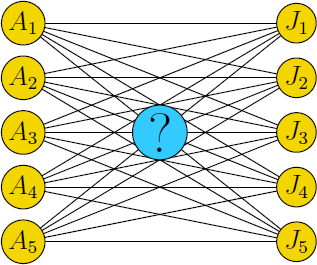
\includegraphics[scale=0.5]{assignmentproblem.png}
\end{figure}
\end{frame}

\begin{frame}
\begin{columns}
\column{0.5\textwidth}
В качестве $A$ и $J$ могут выступать
\begin{itemize}
\item Работники и работы
\item Транспорт и маршруты
\item многое другое
\end{itemize}
\column{0.5\textwidth}
\begin{figure}
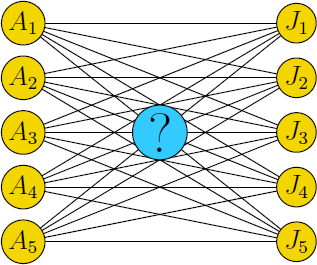
\includegraphics[scale=0.5]{assignmentproblem.png}
\end{figure}
\end{columns}
\end{frame}

\begin{frame}{расширение задачи о назначениях }
Естественное расширение задачи о наздачениях -- переход к трехиндексной постановке.
\end{frame}

\begin{frame}{Сложность}
\begin{columns}
\column{0.5\textwidth}
\begin{figure}
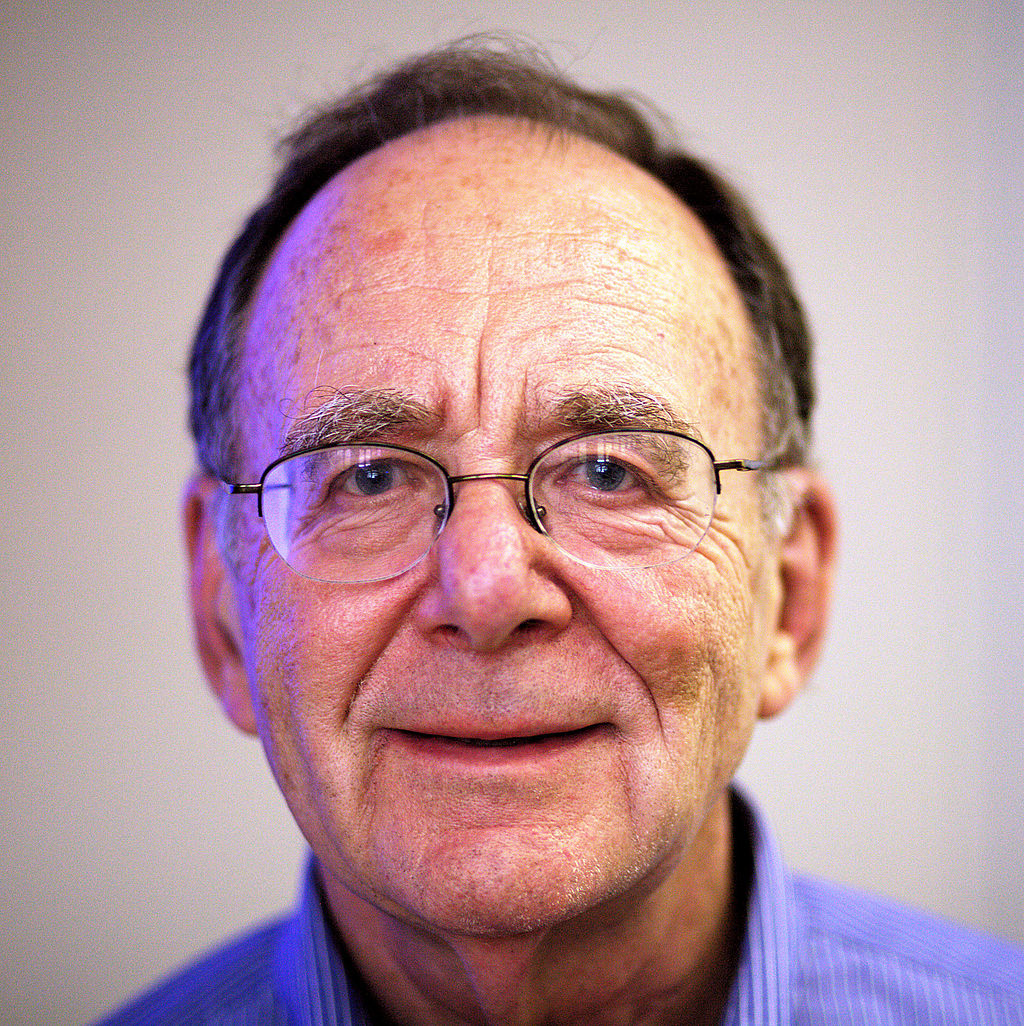
\includegraphics[scale=0.15]{karp.jpg}
\caption{Ричард Мэннинг Карп(03.01.1935)}
\end{figure}
\column{0.5\textwidth}
В 1971 Карп установил, что данная задача относится к классу $\mathcal{NP}$ полных. \\
Задача не может быть решена за полиномиальное время
\end{columns}
\end{frame}

\begin{frame}{Приближенные алоритмы}
Зачастую, достаточно получить решение с определенной точностью. 
Тогда возможно построение полиномиальных алгоритмов. \\
Они не идеальны. 
\end{frame}

\begin{frame}{Цель работы}
\begin{itemize}
\item Исследовать
\item Модифицировать
\end{itemize}
эвристический (приближенный) алгоритм решения 3-ЗОН, основанного на сведении 
задачи к двухиндексной с использованием перестановок. 
\end{frame}

\begin{frame}{Задачи}
\begin{itemize}
\item Изучить математическую модель 3-АЗОН
\item Изучить и проанализировать метод метод, сводящий задачу к двухиндексной
\item Разработать модификации данного алгоритма
\item Программно реализовать данный алгоритм и провести вычислительный эксперимент
\end{itemize}
\end{frame}

\begin{frame}{Постановка 3-АЗОН}
\begin{eqnarray*}
  & \min \displaystyle \sum^n_{i = 1} \displaystyle \sum^n_{j = 1} \displaystyle \sum^n_{k = 1}
  c_{ijk} x_{ijk} \\
  \text{ограничения}
  &\displaystyle \sum^n_{i = 1} \displaystyle \sum^n_{k = 1} x_{ijk} = 1  &(j = 1, \ldots, n) \\
  &\displaystyle \sum^n_{j = 1} \displaystyle \sum^n_{k = 1} x_{ijk} = 1  &(i = 1, \ldots, n) \\
  &\displaystyle \sum^n_{i = 1} \displaystyle \sum^n_{j = 1} x_{ijk} = 1  &(k = 1, \ldots, n) \\
  & x_{ijk} \in \{ 0, 1 \} &(i,j,k = 1, \ldots, n)
\end{eqnarray*}
$c_{ijk} \in C$, где $C$ -- матрица весовых коэфициентов, \\
$x_{ijk} \in X$, где $X$ -- матрица назначений
\end{frame}


\begin{frame}{Постановка 3-АЗОН}
3-АЗОН состоит в том, чтобы выбрать среди элементов трехмерной матрицы $C={c_{ijk}}$ такие $n$ элементов, что сумма в каждом выбраном сечении (для каждой фиксированной переменной $i$, или $j$,или $k$) минимальной. 
\end{frame}

\begin{frame}{Назначение}
Введем понятие назначения. Мы можем
представлять назначение как некое биективное отображение $\varphi$, которое ставит
элементы конечного множества $\mathrm{U}$ в соотвествие элементам конечного
множества $\mathrm{V}$. В тоже время назначение является перестановкой, которая записывается
в виде

\[
\left (
  \begin{tabular}{cccc}
  1 & 2 & \ldots & n\\
  $\varphi (1)$ & $\varphi (2)$ & \ldots & $\varphi (n)$
  \end{tabular}
\right )
\]
\end{frame} 

\begin{frame}{Назначение}
Каждой перестановке множества $\{1, 2, \ldots , n \}$ соответсвует единственная матрица
перестановок $\mathrm{X}_\varphi \in \mathrm{Matrix}_{n \times n}$
\end{frame}

\begin{frame}{Исходный алгоритм}
\end{frame}

\begin{frame}{Достоинства}
Пусть весовые коэфициенты $c_{ijk} \in C$ лежат в отрезке $[a_n, b_n]$, $a_n>0$, $M_n$ -- множество всех возможных $C$. Тогда
\begin{block}{Теорема}
При $b_n / a_n = o(n/ \mathrm{ln} n)$ алгоритм является ассимптотически оптимальным для 3-АЗН на классе матриц $M_n$
и его временная сложность  $O(n^2)$.
\end{block}
\begin{block}{Теорема}
При $b_n / a_n = o(\mathrm{ln} n)$ алгоритм является ассимптотически оптимальным для 3-АЗН на классе матриц $M_n$
и его временная сложность  $O(n \mathrm{ln} n)$. 
\end{block}
\end{frame}

\begin{frame}{Недостатки}
\begin{itemize}
\item Зависит от начальной перестановки.
\item Асимптотическая сходимость при $n \rightarrow \infty$ не имеет практического смысла. 
\end{itemize}
\end{frame}

\begin{frame}{Модификации}
Алгоритм А запускается итеративно. \\
После выполнения выбирается лучший прогон
\end{frame}

\begin{frame}{Модификации}
1. Запускаем алгоритм итеративно \\
2. Запоминаем перестановку после первого цикла \\ 
3. Выбираем случайным образом 2 элемента перестановки и меняем их местами
4. Если решение улучшилось, идем на 2, иначе на 1.
\end{frame}

\begin{frame}{Вычислительный эксперимент}

\end{frame}
\end{document}
